\documentclass[a4paper,12pt]{article}


\usepackage[T1]{fontenc}
\usepackage[utf8]{inputenc}
\usepackage[frenchb]{babel}


\usepackage{graphicx}
\usepackage{xspace}





\title{\Large Compte rendu de travaux pratiques\\ Étude d'un ensemble d'échantillon à l'aide d'un Microscope Électronique à Balayage}

\author{Vincent Denechaud, Olivier Maillet, Alice Odier, Félix Tora}
\date{Vendredi 24 janvier 2014}

\newcommand\ett{Everhart et Thornley\xspace}




\begin{document}

\maketitle


\vfill

\tableofcontents

\newpage


La microscopie électronique est une des techniques importantes de caractérisation d'échantillon. En effet, elle permet d'avoir accès à un grand nombre d'informations. Ce TP est une introduction à l'utilisation du MEB, il permet de mesurer l'ampleur des possibilités d'observation qu'offre ce type de microscopie et de comprendre les raisonnements permettant d'interpréter les clichés obtenus. C'est pour cela que l'on commencera par introduire les différents électrons mis en jeu et leurs détecteurs associés, pour ensuite s'intéresser aux clichés effectués durant la séance et à l'utilisation de photons X dans l'enceinte du MEB pour compléter les informations disponibles.



\section{Rappel sur les différentes sources électroniques et leur détection}


\subsection{Les différentes sources électroniques du MEB}

Des électrons sont accélérés depuis la cathode vers l'échantillon que l'on souhaite étudier. Du fait de leur énergie cinétique, les électrons pénètrent dans la matière de l'échantillon en formant ce que l'on appelle une poire d'interaction (figure \ref{fig:poire_int}).

\begin{figure}[h]
\centering
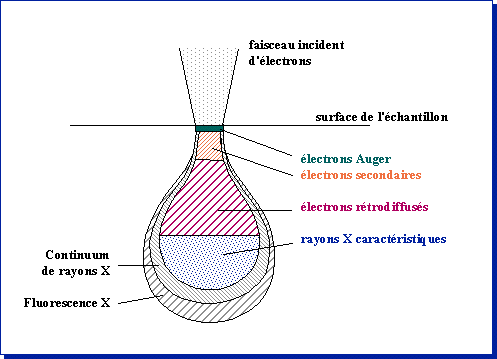
\includegraphics[width = 0.8 \textwidth]{images/poire_int.png}
\caption{Poire d'interaction : on distingue les différents type de rayonnements issus de l'interaction entre le faisceau électronique incident et l'échantillon.}
\label{fig:poire_int}
\end{figure}


En réponse à cette excitation, la matière revient à l'équilibre en émettant du rayonnement X ainsi que des électrons, 
de sorte que le cortège électronique des atomes composant l'échantillon possède une configuration d'équilibre énergétique. 
On peut classer les émissions électroniques selon différentes catégories.

\subsubsection*{Électrons rétro-diffusés}
Lorsque les électrons viennent interagir avec l'échantillon, ils sont, pour la plupart, rétro-diffusés de manière élastique.
Autrement dit, ces électrons interagissent avec les noyaux des atomes de l'échantillon de sorte à conserver leur énergie cinétique.
Ainsi, ces électrons ont une grande profondeur d'échappée, un grand libre parcours moyen dans l'échantillon.

De fait, ces électrons sont très sensibles à la composition chimique de l'échantillon, plus particulièrement, 
au numéro atomique Z des atomes constituant l'échantillon.
Les atomes les plus lourds (Z grand) vont ré-émettre plus d'électrons que les atomes plus légers.
Les éléments les plus lourds vont donc apparaître plus brillants et clairs. L'utilisation des électrons rétro-diffusés permet donc d'avoir un contraste chimique sur l'observation de l'échantillon.
Même s'ils ont une grande longueur de pénétration, ces électrons permettent une résolution spatiale (contraste topographique) d'environ $20$nm (figure \ref{fig:poire_int}).
\begin{figure}
\begin{minipage}[c]{.50\linewidth}
\centering
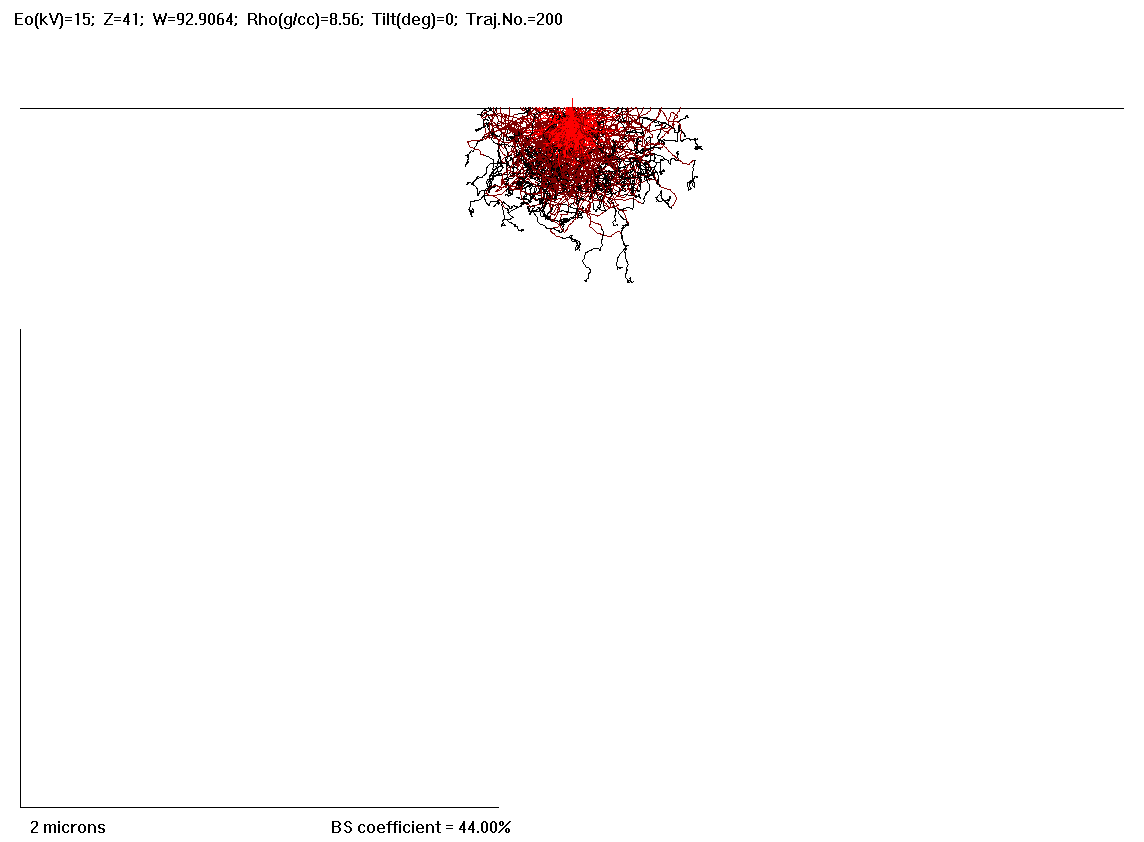
\includegraphics[width = 1 \textwidth]{images/mt_15kv.png}
\end{minipage}
\begin{minipage}[c]{.50\linewidth}
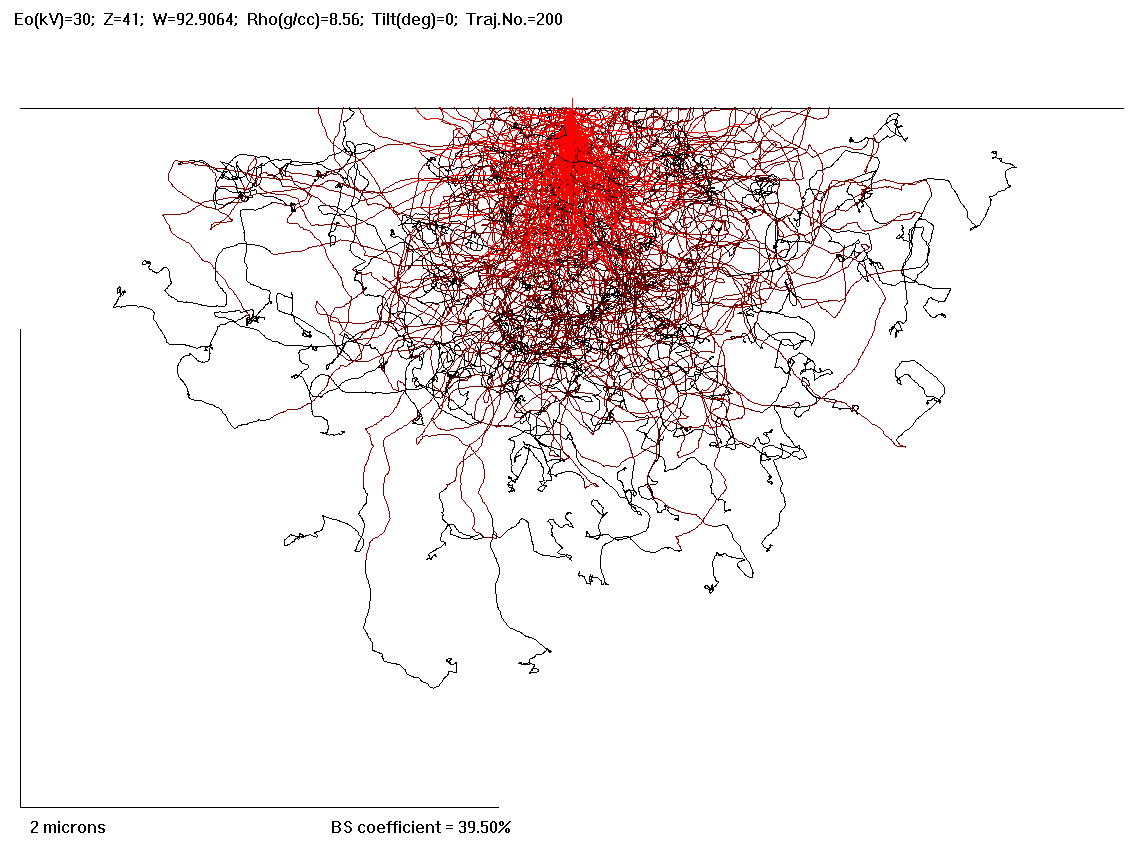
\includegraphics[width = 1 \textwidth]{images/mt_30kv.png}
\end{minipage}
\caption{Trajectoires électroniques empruntées dans l'échantillon, calculées par simulations numériques utilisant une méthode de Monte-Carlo. On constate que la quantité d'électrons rétro-diffusés augmente avec l'énergie du faisceau incident (à gauche $15$kV, à droite $30$kV).}
\label{fig:montecarlo}
\end{figure}

Comme le montre la figure \ref{fig:montecarlo}, un électron pénétrant dans l'échantillon peut emprunter
 avec une probabilité non nulle une trajectoire qui
  ressort de l'échantillon, et ce d'autant plus que son énergie cinétique incidente est grande.

\subsubsection*{Électrons secondaires}
En outre des électrons diffusés de manière quasi-élastique, une autre partie de ces derniers est diffusée de manière inélastique par l'échantillon.
Ce sont les électrons dits secondaires. 
Ces électrons cèdent donc très vite leur énergie cinétique et ont un faible libre parcours moyen ainsi qu'une faible profondeur de pénétration dans l'échantillon. 
Néanmoins, étant donné que ces derniers ressortent très vite de l'échantillon, la résolution spatiale obtenue 
après leur détection est bien meilleure (de l'ordre de $5$nm) que celle obtenue avec les électrons rétro-diffusés.
Les électrons secondaires seront donc très utiles pour réaliser un bon contraste topographique.
On notera cependant qu'il y a beaucoup moins d'électrons du type secondaire que rétro-diffusé. 
L'utilisation des électrons secondaires nécessite donc un temps de pose plus long pour réaliser un cliché.

\subsection{Les techniques de détection associées}

\subsubsection*{Détection des électrons rétro-diffusés}

La détection des électrons rétro-diffusés se fait à l'aide d'un (double) détecteur à semi-conducteur 
(qui n'est généralement rien d'autre qu'une jonction Schottky, cf figure \ref{fig:detect_sc}). 

\begin{figure}[h]
\centering
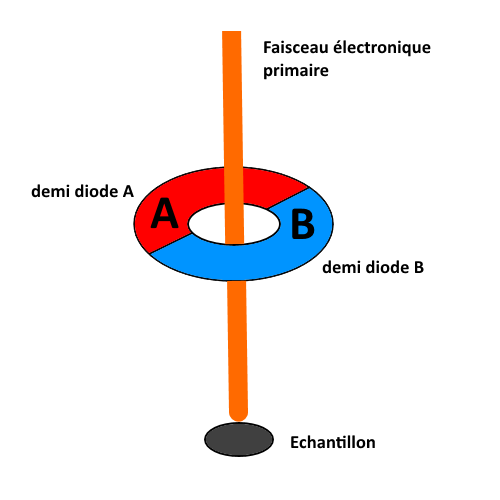
\includegraphics[width = 0.5 \textwidth]{images/detect_sc.png}
\caption{Détecteur à semi-conducteur pour électrons rétro-diffusés. Dans le cas des expériences présentées ici, il s'agit d'un détecteur annulaire positionné dans l'axe du faisceau primaire. On appelle A et B les deux demi-diodes composant le détecteur.}
\label{fig:detect_sc}
\end{figure}


Lorsqu'un électron rétro-diffusé vient frapper la surface semi-conductrice du détecteur, 
et si celui-ci possède une énergie cinétique appropriée,
il y a alors création d'une paire électron-trou dans le semi-conducteur. 
Les porteurs de charge sont alors collectés aux contacts de la jonction, d'où la mesure d'un courant et détection de l'électron rétro-diffusé.

Comme le montre la figure \ref{fig:detect_sc}, le détecteur est composé de deux "demi-diodes".
Un tel découpage permet différents modes de fonctionnement.
En effet, il devient possible de séparer le signal donné par le détecteur en deux voies A et B.

Additionner ou soustraire les signaux A et B permet d'obtenir respectivement un contraste de composition de l'échantillon ou bien topographique, comme indiqué figure \ref{fig:detect_sc_contraste}.

\begin{figure}
\centering
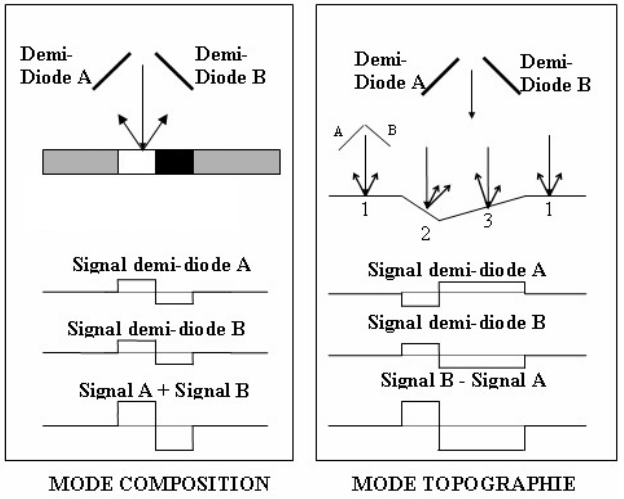
\includegraphics[width = 0.9 \textwidth]{images/detect_sc_contraste.png}
\caption{Contrastes de composition et topographique obtenus en manipulant les voies A et B du détecteur à électrons rétro-diffusés.}
\label{fig:detect_sc_contraste}
\end{figure}







\subsubsection*{Détection des électrons secondaires}

La détection des électrons rétro-diffusés se fait à l'aide du détecteur d'\ett. Il est composé d'une grille, d'un scintillateur et d'un photo-multiplicateur (figure \ref{fig:detect_ett}).

\begin{figure}
\centering
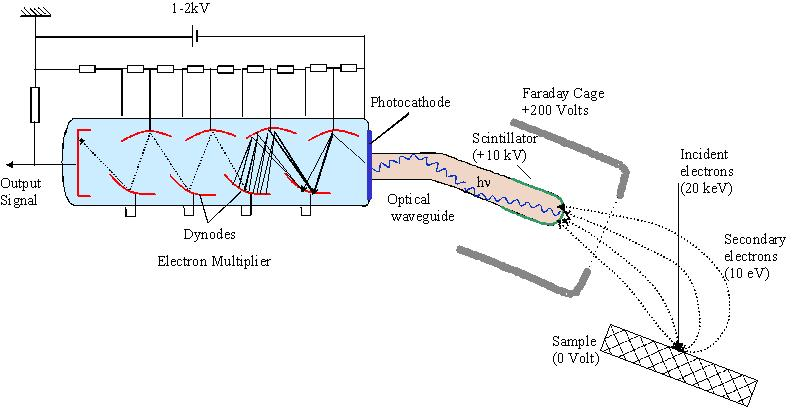
\includegraphics[width = 0.9 \textwidth]{images/detect_ett.png}
\caption{Détecteur d'\ett composé d'un collecteur, d'un scintillateur et d'un photo-multiplicateur.}
\label{fig:detect_ett}
\end{figure}
 
On polarise le collecteur en tension à $+200$ Volts, ce qui a pour rôle d'attirer les électrons secondaires. 
Cette grille joue aussi le rôle de "cage de Faraday", ce qui permet de ne pas attirer des électrons du faisceau incident. 
Les électrons secondaires possédant une faible énergie, ils sont ainsi sélectionnés par rapport aux électrons rétro-diffusés.
Il reste néanmoins les électrons rétro-diffusés avec l'angle solide correspondant à la direction du détecteur d'\ett dont l'on ne peut pas s'affranchir. 

Une fois les électrons collectés, ils sont accélérés vers un scintillateur polarisé à $10$kV qui les "transforme" en photons.
Ces photons sont ensuite conduits vers un photo-multiplicateur qui a pour but d'amplifier le signal final obtenu.


Il est possible d'utiliser le détecteur d'\ett  pour détecter les électrons rétro-diffusés.
En effet, en polarisant négativement le collecteur, les électrons secondaires émis à la surface de l'échantillon sont repoussés.
Ainsi, on ne détecte que les électrons rétro-diffusés possédant l'angle solide associé à la position du détecteur d'\ett, dit électrons rétro-diffusés à incidence rasante.
Une telle manipulation permet d'obtenir des informations complémentaires sur le contraste topographique.


\subsection{Grandissement et mise au point}
Pour le MEB, le grandissement n'est pas dû aux lentilles comme dans les microscopes optiques traditionnels, mais à la taille de la zone de balayage. Plus la zone de balayage est petite plus le grandissement sera grand. Le réglage de la netteté ne se fait donc pas comme en optique en déplaçant les lentilles. Ici, c'est le rapport entre la taille du faisceau et la taille de la zone de balayage qui définit la netteté. Pour que l'image soit nette, il faut que la taille du faisceau soit plus petite que le pas de balayage, ceci permet d'éviter tout recouvrement. On cherche donc à focaliser de manière à remplir cette condition et cela se fait en changeant la focale des lentilles. En effet, comme ce sont des lentilles électromagnétiques, leur focale peut être changée en modifiant le courant qui les traverse.


C'est le fait que le grandissement ne dépendent pas des lentilles qui permet d'avoir une résolution bien plus grande. Comme la distance de travail est beaucoup plus grande qu'en optique et donc l'angle bien plus petit, on obtient des profondeurs de champs plus importante qu'en microscopie optique. 



\section{Échantillon d'une éponge de nickel}

L'observation de ce premier échantillon, une éponge de nickel, va nous permettre d'illustrer l'utilisation des différentes techniques présentées précédemment.

\subsection{Détecteur d'\ett}

Utilisant comme technique d'imagerie initiale les électrons secondaires recueillis par le détecteur d'\ett,
on accède à une première observation de l'échantillon présentée figure \ref{fig:ni_es}. 

\begin{figure}[h]
\centering
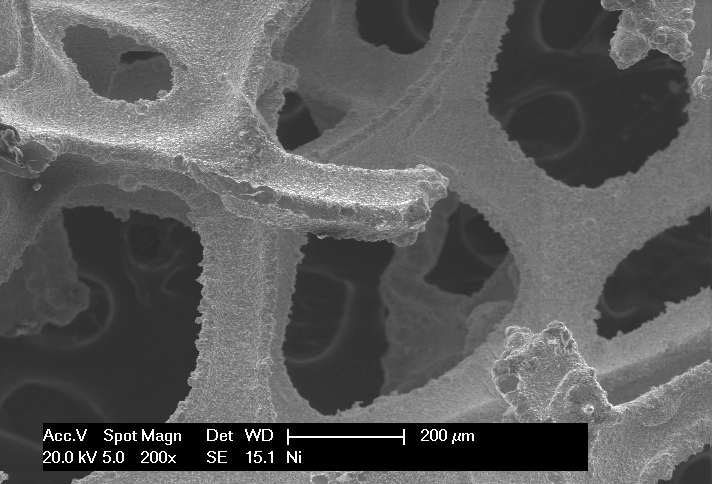
\includegraphics[width = 0.7 \textwidth]{images/ni_es.png}
\caption{Observation de l'éponge de nickel utilisant les électrons secondaires recueillis par le détecteur d'\ett. L'échantillon est ici grossi 200 fois.}
\label{fig:ni_es}
\end{figure}

Comme déjà évoqué,
cette technique a l'avantage d'offrir une grande profondeur de champ à l'image obtenue contrairement aux microscopies optiques. Cette première technique d'imagerie permet un contraste de profondeur de champ et donc de visualiser spatialement la forme de l'échantillon.

Le détecteur d'\ett permet aussi de récolter des électrons rétro-diffusés. Ces électrons rétro-diffusés sont
collectés dans un angle solide bien précis, ainsi l'image obtenue à l'aide de cette technique présente une
certaine profondeur de champ mais aussi des effets d'ombre et de lumière. Ces effets sont dus à l'angle
d'incidence des électrons collectés. L'image obtenue à l'aide de cette technique est présentée figure
\ref{fig:ni_er_rasant}.

\begin{figure}[h!]
\centering
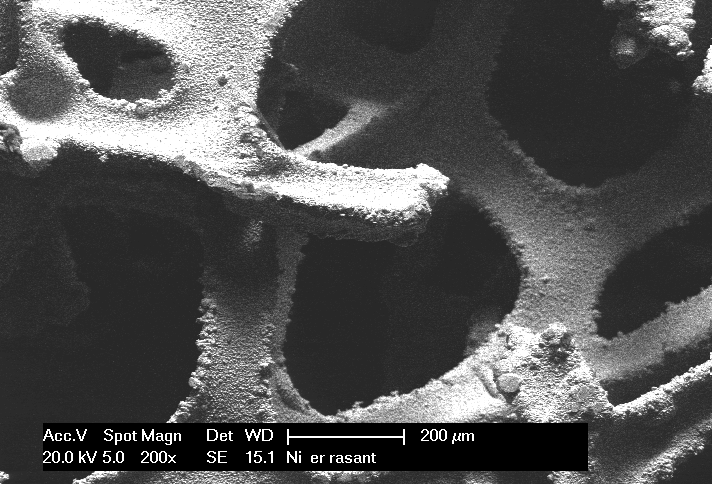
\includegraphics[width = 0.7 \textwidth]{images/ni_er_rasant.png}
\caption{Observation de l'éponge de nickel utilisant les électrons rétro-diffusés recueillis par le détecteur d'\ett. L'échantillon est ici grossi 200 fois.}
\label{fig:ni_er_rasant}
\end{figure}

\clearpage

\subsection{Détecteur à semi-conducteur}

L'utilisation du détecteur à semi-conducteur permet de collecter un grand nombre d'électrons rétro-diffusés
et d'obtenir deux types d'imagerie. L'utilisation du mode $A+B$ permet d'obtenir une image avec un contraste
en composition chimique. L'image de l'éponge de nickel obtenue avec cette technique est présentée à la figure
\ref{fig:ni_er_apb_amb}. Sur cette image on voit que la profondeur de champ du cliché est très faible. Cependant
le contraste en composition chimique permet d'obtenir d'autres informations tout aussi importantes.


On peut voir sur l'échantillon certaines excroissances qui apparaissent plus foncées. Cette image permet d'observer
la présence d'impuretés sur le matériau, tout du moins de parties faites d'éléments différents.


\begin{figure}
\begin{minipage}[c]{.5\linewidth}
\centering
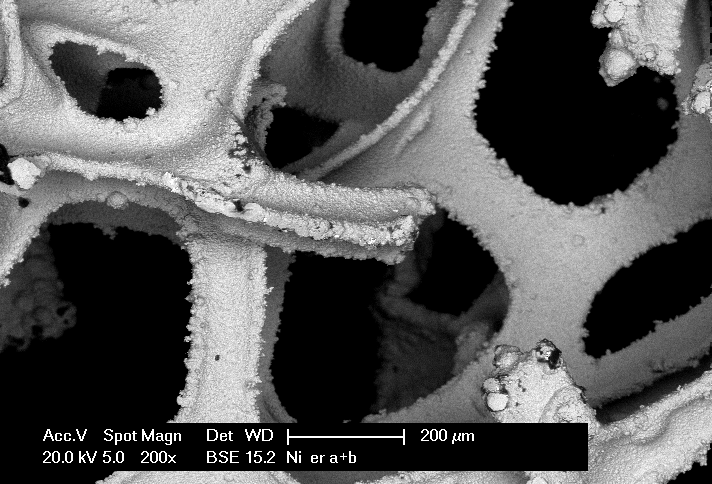
\includegraphics[width = 1 \textwidth]{images/ni_er_apb.png}
\end{minipage}
\begin{minipage}[c]{.5\linewidth}
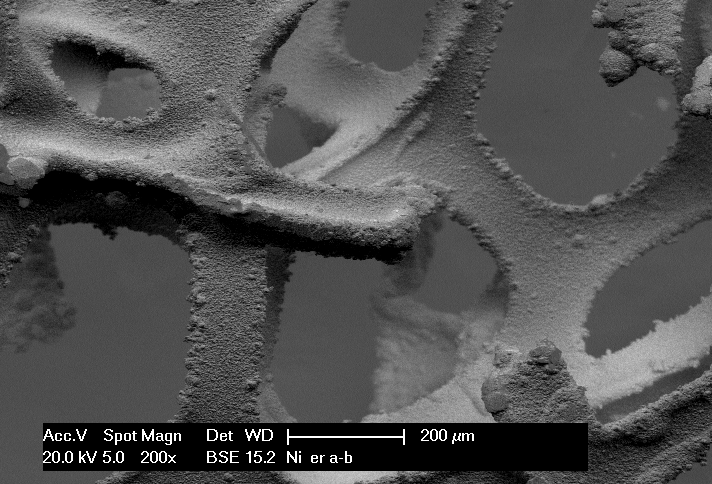
\includegraphics[width = 1 \textwidth]{images/ni_er_amb.png}
\end{minipage}
\caption{Observation de l'éponge de nickel utilisant les électrons rétro-diffusés recueillis par le détecteur à semi-conducteur en mode $A+B$ et $A-B$. L'échantillon est ici grossi 200 fois.}
\label{fig:ni_er_apb_amb}
\end{figure}

On peut voir sur l'échantillon certaines excroissances qui apparaissent plus foncées. Cette image permet d'observer
la présence d'impuretés sur le matériau, tout du moins de parties faites d'éléments différents.


Le détecteur à semi-conducteur permet également de réaliser un cliché différent en utilisant les mêmes électrons
rétro-diffusés. L'image réalisée avec le mode $A-B$ est présentée sur la figure \ref{fig:ni_er_apb_amb}. Sur ce cliché
le contraste est topographique.


 

\section{Échantillon de silicium}

\subsection{Détecteur d'\ett}

On réalise une image de l'échantillon de silicium en collectant les électrons secondaires avec le détecteur d'\ett.
Le cliché obtenu est présenté sur la figure \ref{fig:si_es}. On garde à l'esprit qu'il présente un contraste topographique.
On observe des structures pyramidales en bas-relief ou en haut-relief. Les conditions d'éclairage du cliché ne permettent
pas d'opter pour l'une ou l'autre des solutions (bas-relief ou haut-relief). Quoiqu'il en soit, l'observation de ce cliché nous permet de penser que la structure de l'échantillon est cristalline, étant donné la relative périodicité des motifs observés.

\begin{figure}[h]
\centering
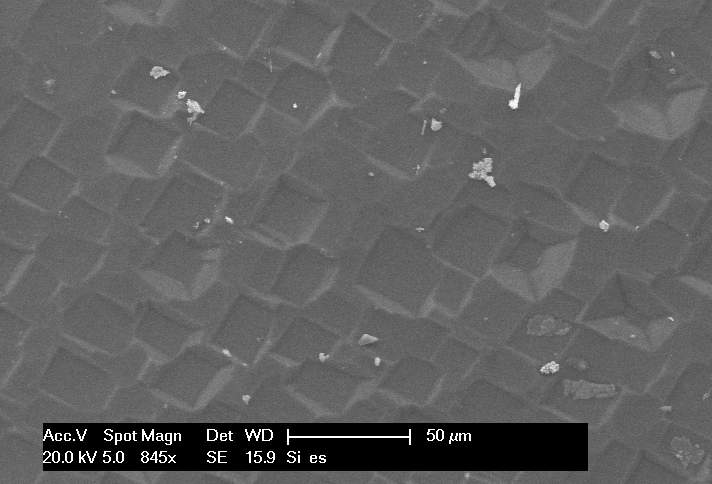
\includegraphics[width=0.7\textwidth]{images/si_es.png}
\caption{Observation d'un échantillon de silicium utilisant les électrons secondaires collectés dans le détecteur d'\ett. L'échantillon est ici grossi 845 fois.}
\label{fig:si_es}
\end{figure}

Afin de déterminer si les pyramides sont en bas-relief ou non, on utilise un autre cliché. La figure \ref{fig:si_er_rasant} présente
un cliché réalisé à l'aide du détecteur de \ett mais en collectant les électrons rétro-diffusés. Les électrons utilisés étant rasants,
on observe des effets d'ombre et de lumière. Par exemple une poussière en haut à droite du cliché projette son ombre vers le bas.
On en déduit que l'éclairage provient du haut du cliché. Ainsi, il est maintenant possible de se prononcer sur l'enfoncement des pyramides.
Les faces éclairées sont celles situées en bas, ce qui veut dire que les pyramides sont en bas-relief.

\begin{figure}
\centering
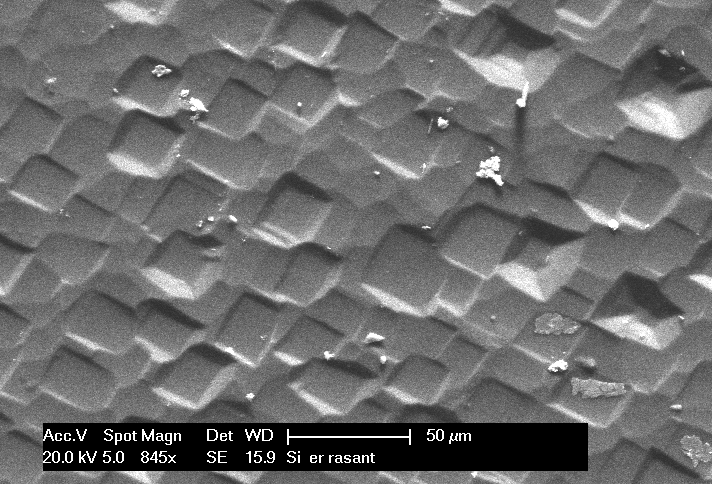
\includegraphics[width=0.7\textwidth]{images/si_er_rasant.png}
\caption{Observation d'un échantillon de silicium utilisant les électrons rétro-diffusés collectés dans le détecteur d'\ett. L'échantillon est ici grossi 845 fois.}
\label{fig:si_er_rasant}
\end{figure}

\subsection{Détecteur à semi-conducteur}

En utilisant le détecteur à semi-conducteur en mode $A+B$, on observe sur la figure \ref{fig:si_er_apb_amb} les contrastes de compositions et, en l'occurrence, qu'il y a deux types de poussières. Mais le plus important pour la détermination de la structure cristallographique est le mode $A-B$. En effet, cela permet de gommer la composition chimique et d'avoir ainsi accès au relief résiduel. On observe sur la figure \ref{fig:si_er_apb_amb} des carrés, ce qui implique une symétrie $\frac{\pi}{2}$ et donc, un axe d'ordre 4. L'orientation du cristal est donc selon le plan (100) ou (010). En effet, une orientation selon le plan (110), on aurait eu un axe d'ordre 3 et donc des formes hexagonales sur le cliché.
\begin{figure}
\begin{minipage}[c]{.5\linewidth}
\centering
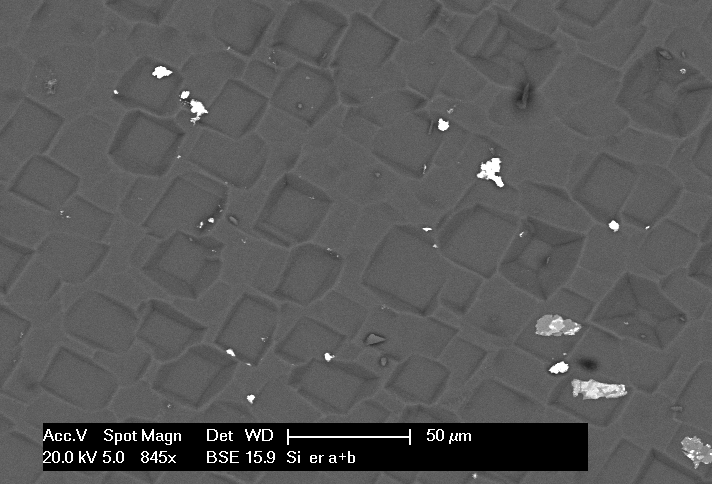
\includegraphics[width=1\textwidth]{images/si_er_apb.png}
 \end{minipage}\hfill
\begin{minipage}[c]{.5\linewidth}
\centering
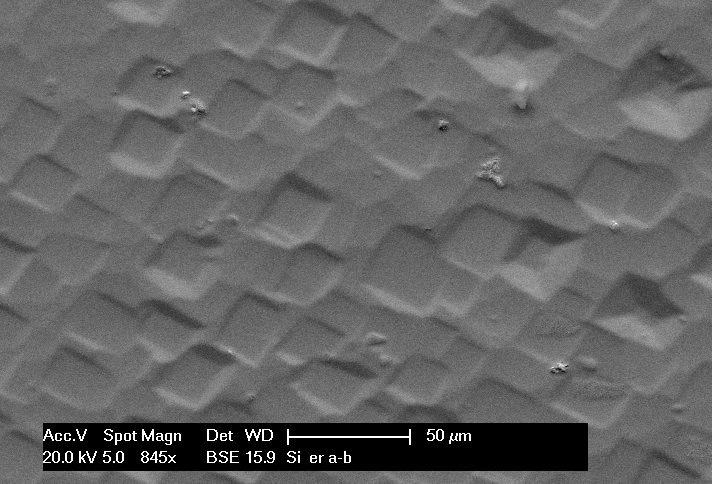
\includegraphics[width=1\textwidth]{images/si_er_amb.png}
\end{minipage}
\caption{Observation d'un échantillon de silicium utilisant les électrons rétro-diffusés recueilli par le détecteur semi-conducteur en mode $A+B$ et $A-B$. L'échantillon est ici grossi 845 fois.}
\label{fig:si_er_apb_amb}
\end{figure}

\section{Échantillon d'aluminium}


Cet échantillon est la résultante d'un morceau d'aluminium brisé, on peut voir à l'œil une rugosité importante. Quelles sont les informations que pourra nous donner une étude au microscope MEB.

\subsection{Détecteur d'\ett}
Avec les électrons secondaires, on voit sur l'échantillon deux types de reliefs. Des déchirures à certains endroit, avec des facettes acérées et des gouffres remplis de boules comme on peut le voir dans la figure \ref{fig:alu_reliefs}. Les deux types de ruptures dans ce même échantillon peuvent être expliqués à l'aide d'un diagramme de phase (figure \ref{fig:diagphase}).

\begin{figure}
\begin{minipage}[c]{.5\linewidth}
\centering
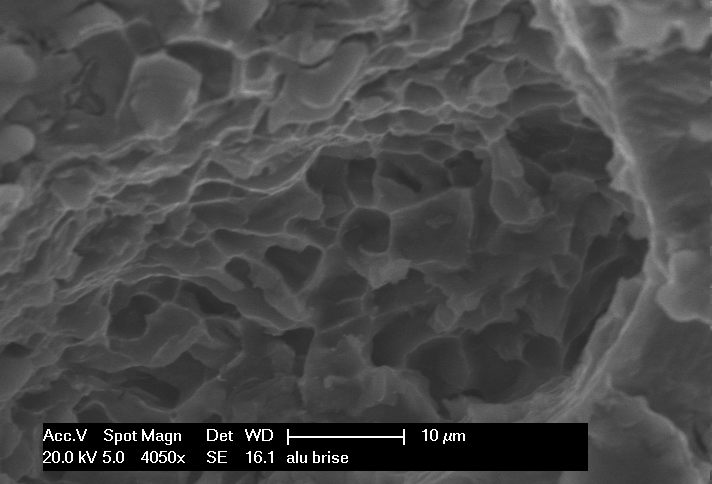
\includegraphics[width=1\textwidth]{images/alu_arretes.png}
 \end{minipage}\hfill
\begin{minipage}[c]{.5\linewidth}
\centering
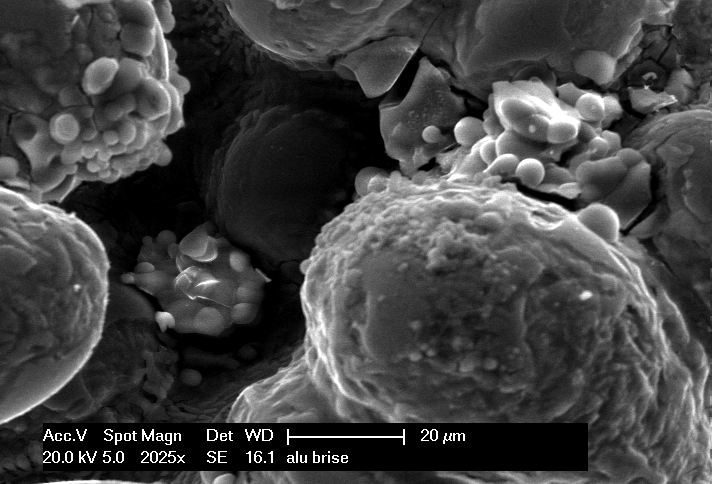
\includegraphics[width=1\textwidth]{images/alu_brise.png}
\end{minipage}
\caption{Observation de l'échantillon d'aluminium en utilisant les électrons secondaires}
\label{fig:alu_reliefs}
\end{figure}


En effet, il y a initialement dans cet échantillon 7\% de Si. Sur le diagramme de phase, on voit qu'il n'y a pas de composé défini. A l'eutectique, il y a donc deux phases démixées, d'où la présence de petits grains de Si entourés d'aluminium. Les trous sont dûs au retrait volumique de la solution eutectique. La fracture se fait donc soit dans le trous soit où il y a déchirure. C'est la marque d'un comportement ductile: le matériau s'étire puis casse au niveau des arêtes. On voit aussi des dendrites sur la figure \ref{fig:dendrites} qui viennent de la solidification dans la phase liquide à partir d'un germe solide.



\begin{figure}[h!]
\centering
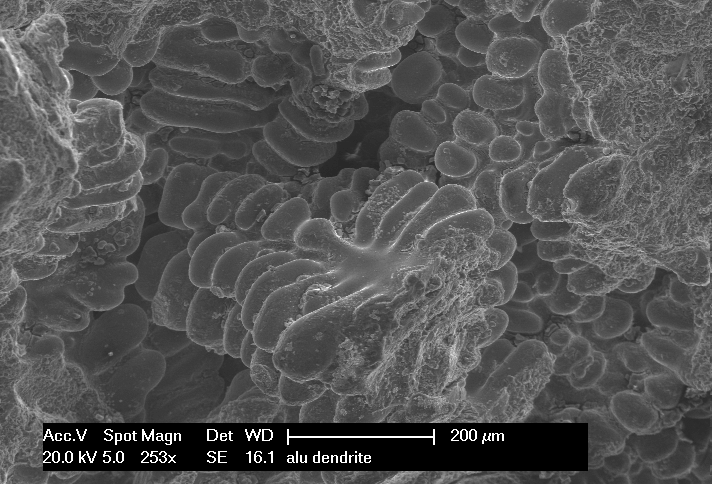
\includegraphics[width=0.7\textwidth]{images/alu_dendrites.png}
\caption{Observation des dendrites à l'aide des électrons secondaire. Le grossissement est de 253.}
\label{fig:dendrites}
\end{figure}

\subsection{Détecteur à semi-conducteur}

Lorsqu'on utilise les électrons rétro-diffusés, on ne peut voir le contraste chimique à cause des reliefs trop important. On ne peut donc pas conclure sur la topographie de la structure eutectique. 

\begin{figure}[h]
\centering
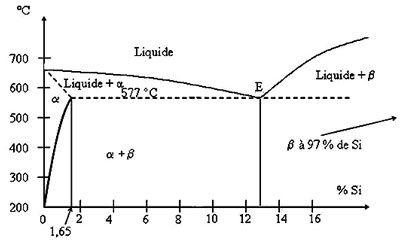
\includegraphics[width=0.7\textwidth]{images/diagphasealusi.jpg}
\caption{Diagramme de phase de l'alliage Aluminium Silicium.}
\label{fig:diagphase}
\end{figure}


\section{Échantillon d'aluminium poli}

Cet échantillon possède une composition identique à l'alliage étudié dans la section précédente (à savoir, un alliage d'aluminium et de silicium). 
Il a été refroidi à haute pression puis poli.
Des fibres (métalliques) ont été introduites dans l'alliage avant la solidification afin de le rendre plus solide.

\subsection{Détecteur d'\ett}

Étudions, tout d'abord, l'échantillon à l'aide des électrons recueillis par le détecteur d'\ett. 
La figure \ref{fig:alu_poli_es} montre le cliché obtenu avec les électrons secondaires.
On peut distinguer le contour des fibres introduites dans l'alliage, mais le contraste de l'image laisse 
à désirer.

\begin{figure}[h]
\centering
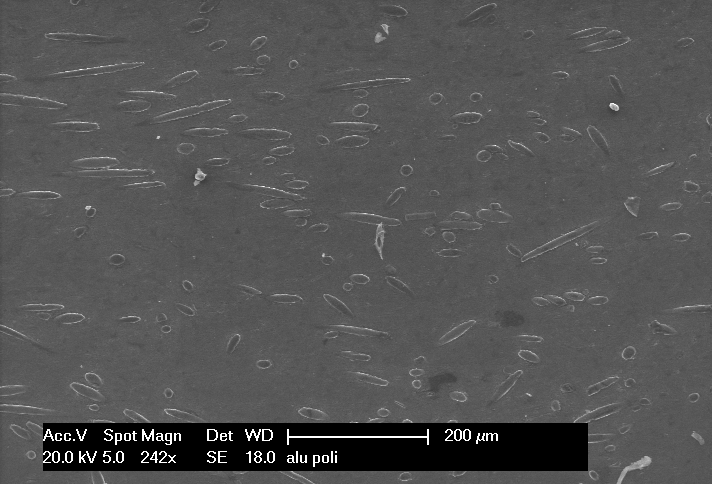
\includegraphics[width=0.7\textwidth]{images/alu_es.png}
\caption{Observation de l'échantillon d'alliage d'aluminium avec fibres en utilisant les électrons secondaires.}
\label{fig:alu_poli_es}
\end{figure}

De meilleurs résultats sont obtenus en utilisant les électrons rétro-diffusés à incidence rasante, indiqué figure \ref{fig:alu_poli_er_rasant}.
Ce cliché indique que les fibres sont en relief par rapport à la coupe, ce qui sous entend que ces fibres plus dures que l'alliage.

\begin{figure}[h!]
\centering
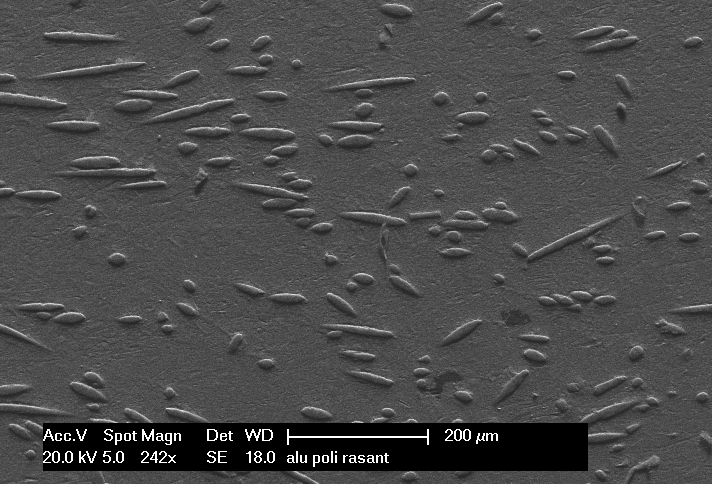
\includegraphics[width=0.7\textwidth]{images/alu_er_rasant.png}
\caption{Observation de l'échantillon d'alliage d'aluminium avec fibres en utilisant les électrons rétro-diffusés à incidence rasante.}
\label{fig:alu_poli_er_rasant}
\end{figure}

\subsection{Détecteur à semi-conducteur}

On utilise maintenant le détecteur à semi-conducteur.
Le mode $A-B$ permet de réaliser un cliché avec un bon contraste topographique (cf figure\ref{fig:alu_poli_a-b}), et confirme bien que les fibres sont en relief par rapport au plan de coupe de l'échantillon.

\begin{figure}[h]
\centering
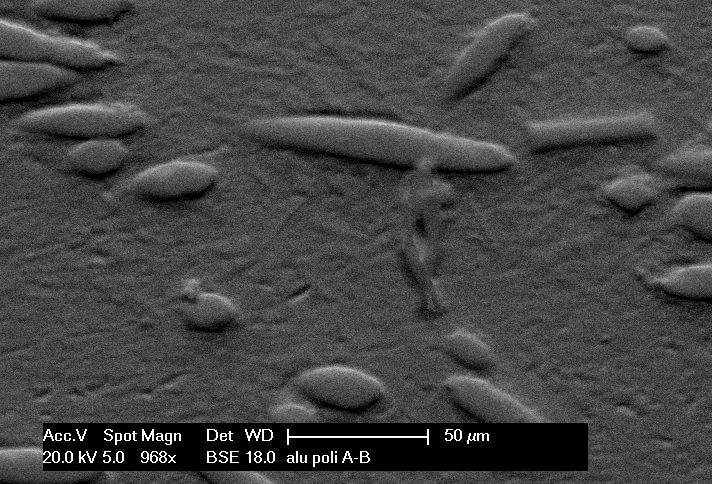
\includegraphics[width=0.7\textwidth]{images/alu_er_amb.png}
\caption{Observation de l'échantillon d'alliage d'aluminium avec fibres en utilisant les électrons rétro-diffusés en mode $A-B$ (contraste topographique).}
\label{fig:alu_poli_a-b}
\end{figure}

Le mode $A+B$ permet d'obtenir un cliché de l'échantillon avec un contraste chimique, comme indiqué sur la figure \ref{fig:alu_poli_a+b}.
Au niveau de l'alliage, on distingue bien deux espèces chimiques différentes, à savoir l'aluminium et le silicium ($Z_{Al}<Z_{Si}$ donc le Si apparaît plus clair que l'Al).
Les fibres apparaissant plus sombres, on en déduit que l'élément que les compose est plus léger, au sens où $Z_{fibre}<Z_{Al}<Z_{Si}$.
Enfin, on peut distinguer sur ces clichés les sillons réalisées par des grains abrasifs lors du polissage de la surface.


\begin{figure}[h!]
\begin{minipage}[c]{.5\linewidth}
\centering
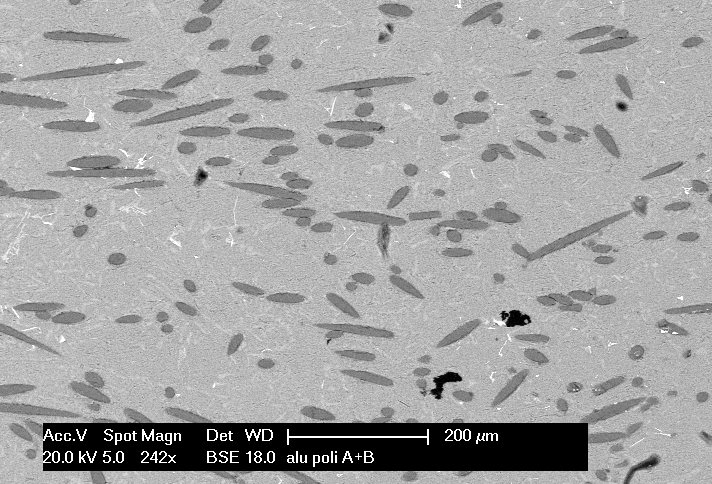
\includegraphics[width=1\textwidth]{images/alu_er_apb.png}
 \end{minipage}\hfill
\begin{minipage}[c]{.5\linewidth}
\centering
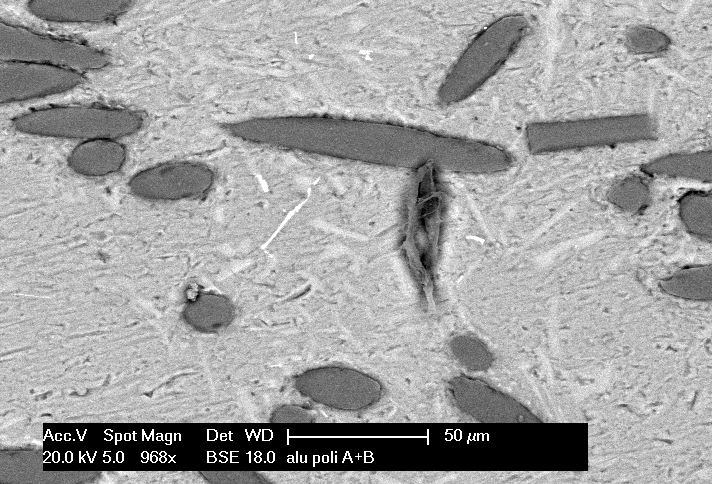
\includegraphics[width=1\textwidth]{images/alu_er_apb_g.png}
\end{minipage}
\caption{Observation de l'échantillon d'alliage d'aluminium avec fibres en utilisant les électrons rétro-diffusés en mode $A+B$ (contraste chimique) pour différentes résolutions.}
\label{fig:alu_poli_a+b}
\end{figure}

\newpage

\section{Microanalyse X EDS}

La structure du dernier échantillon n'est pas connue avant les études effectuées.
L'étude de cet échantillon va permettre de présenter les techniques de microanlyse
X qui permettent de caractériser directement les espèces présentes dans l'échantillon.
La technique de microanalyse utilisée est EDS pour Energy Dispersion System. Le
détecteur collecte des électrons X dont les énergies sont caractéristiques de l'élément
avec lequel ils ont interagis.

L'échantillon est un empilement de couches minces sur un substrat. L'observation de
l'échantillon en mode $A+B$ permet d'observer les différences de composition à l'aide
du contraste chimique. Le cliché réalisé est présenté sur la figure \ref{fig:sec_er_apb}.
La structure couches minces est clairement visible, le contraste chimique ne permet pas
de caractériser complètement l'échantillon. Pour ce faire des informations sur les éléments
qui le compose sont nécéssaires.


\begin{figure}
\centering
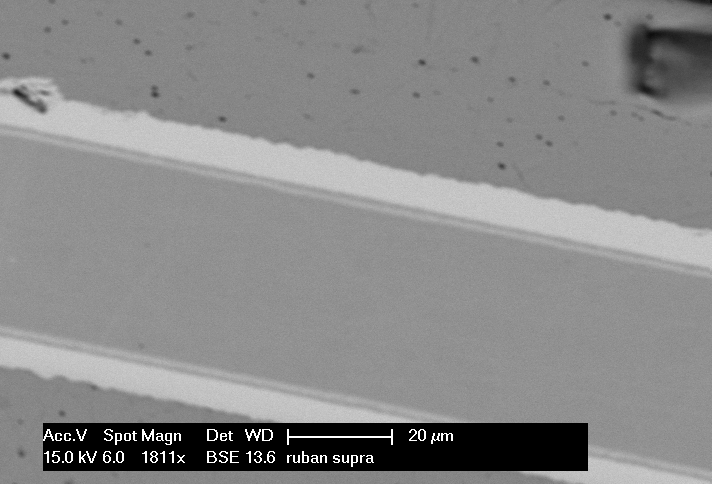
\includegraphics[width=0.7\textwidth]{images/sec_er_apb_1.png}
\caption{Observation en mode $A+B$ de l'échantillon de couches minces. Le contraste chimique permet d'observer les différences de composition. Les techniques de microanalyse X permettrons d'être plus précis.}
\label{fig:sec_er_apb}
\end{figure}



\begin{figure}
\centering
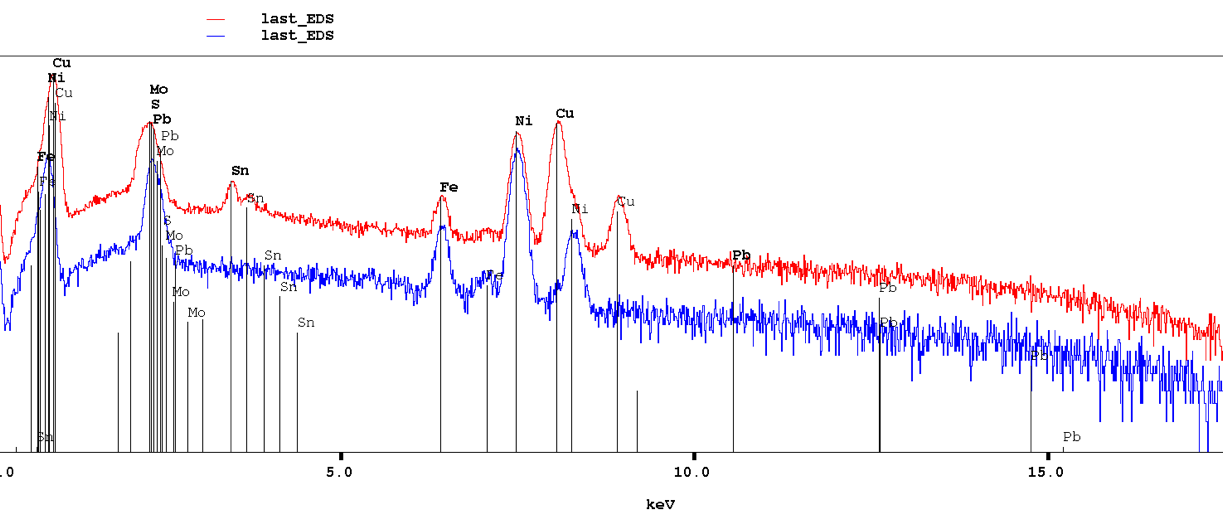
\includegraphics[width=\textwidth]{images/im2.png}
\caption{Spectre EDS au niveau des couches minces du dernier échantillon. Les énergies sont en abscisses l'intensité en ordonnées.}
\label{fig:spectre_1}
\end{figure}

Le spectre obtenu pour les énergies des électrons collectés est présenté à la figure \ref{fig:spectre_1}.
Les éléments dont la présence est suggérée par le spectre sont le fer cuivre, le molybdène, le plomb, le nickel.
On voit cependant apparaître des problèmes de résolution. Le spectre de la figure \ref{fig:spectre_1}
ne permet pas de différencier le molybdène du plomb. Mais l'absence des autres raies de l'élément plomb
permet de conclure positivement quant à la présence de molybdène dans l'échantillon.

Lorsque le faisceau est placé directement sur la couche elle même le spectre obtenu est différent.
Il est présenté à la figure \ref{fig:spectre_2}. On ne trouve alors que deux éléments le molybdène et
l'étain.






\begin{figure}
\centering
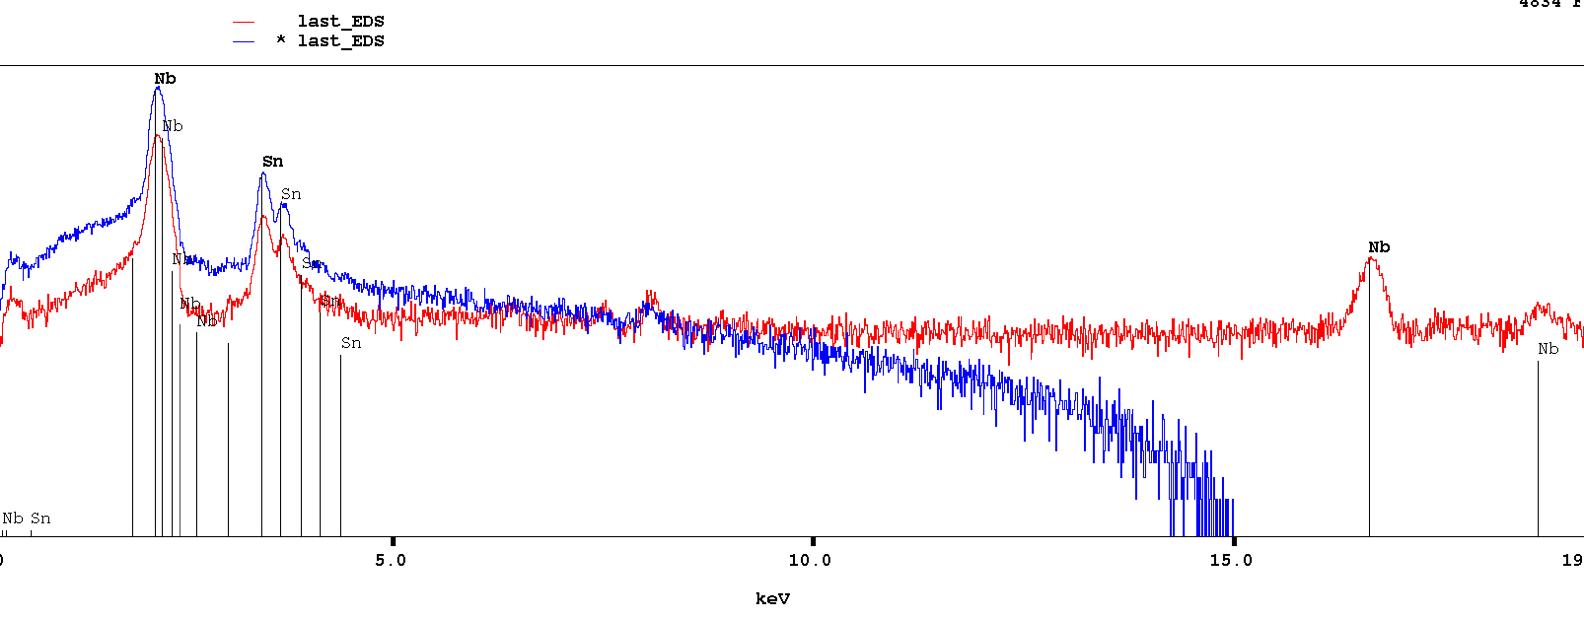
\includegraphics[width=\textwidth]{images/im4.png}
\caption{Spectre EDS au niveau des couches minces du dernier échantillon. Les énergies sont en abscisses l'intensité en ordonnées.}
\label{fig:spectre_2}
\end{figure}

La technique EDS permet de déterminer localement les espèces présentes dans l'échantillon (et ce sur une profondeur
de l'ordre du millimètre). En répétant la mesure en différents lieux on est capable de reconstruire une image
dont les codes couleurs sont en fait la signature d'un élément en particulier. Un tel cliché a été réalisé et le
résultat est présenté figure \ref{fig:eds}.



\begin{figure}
\centering
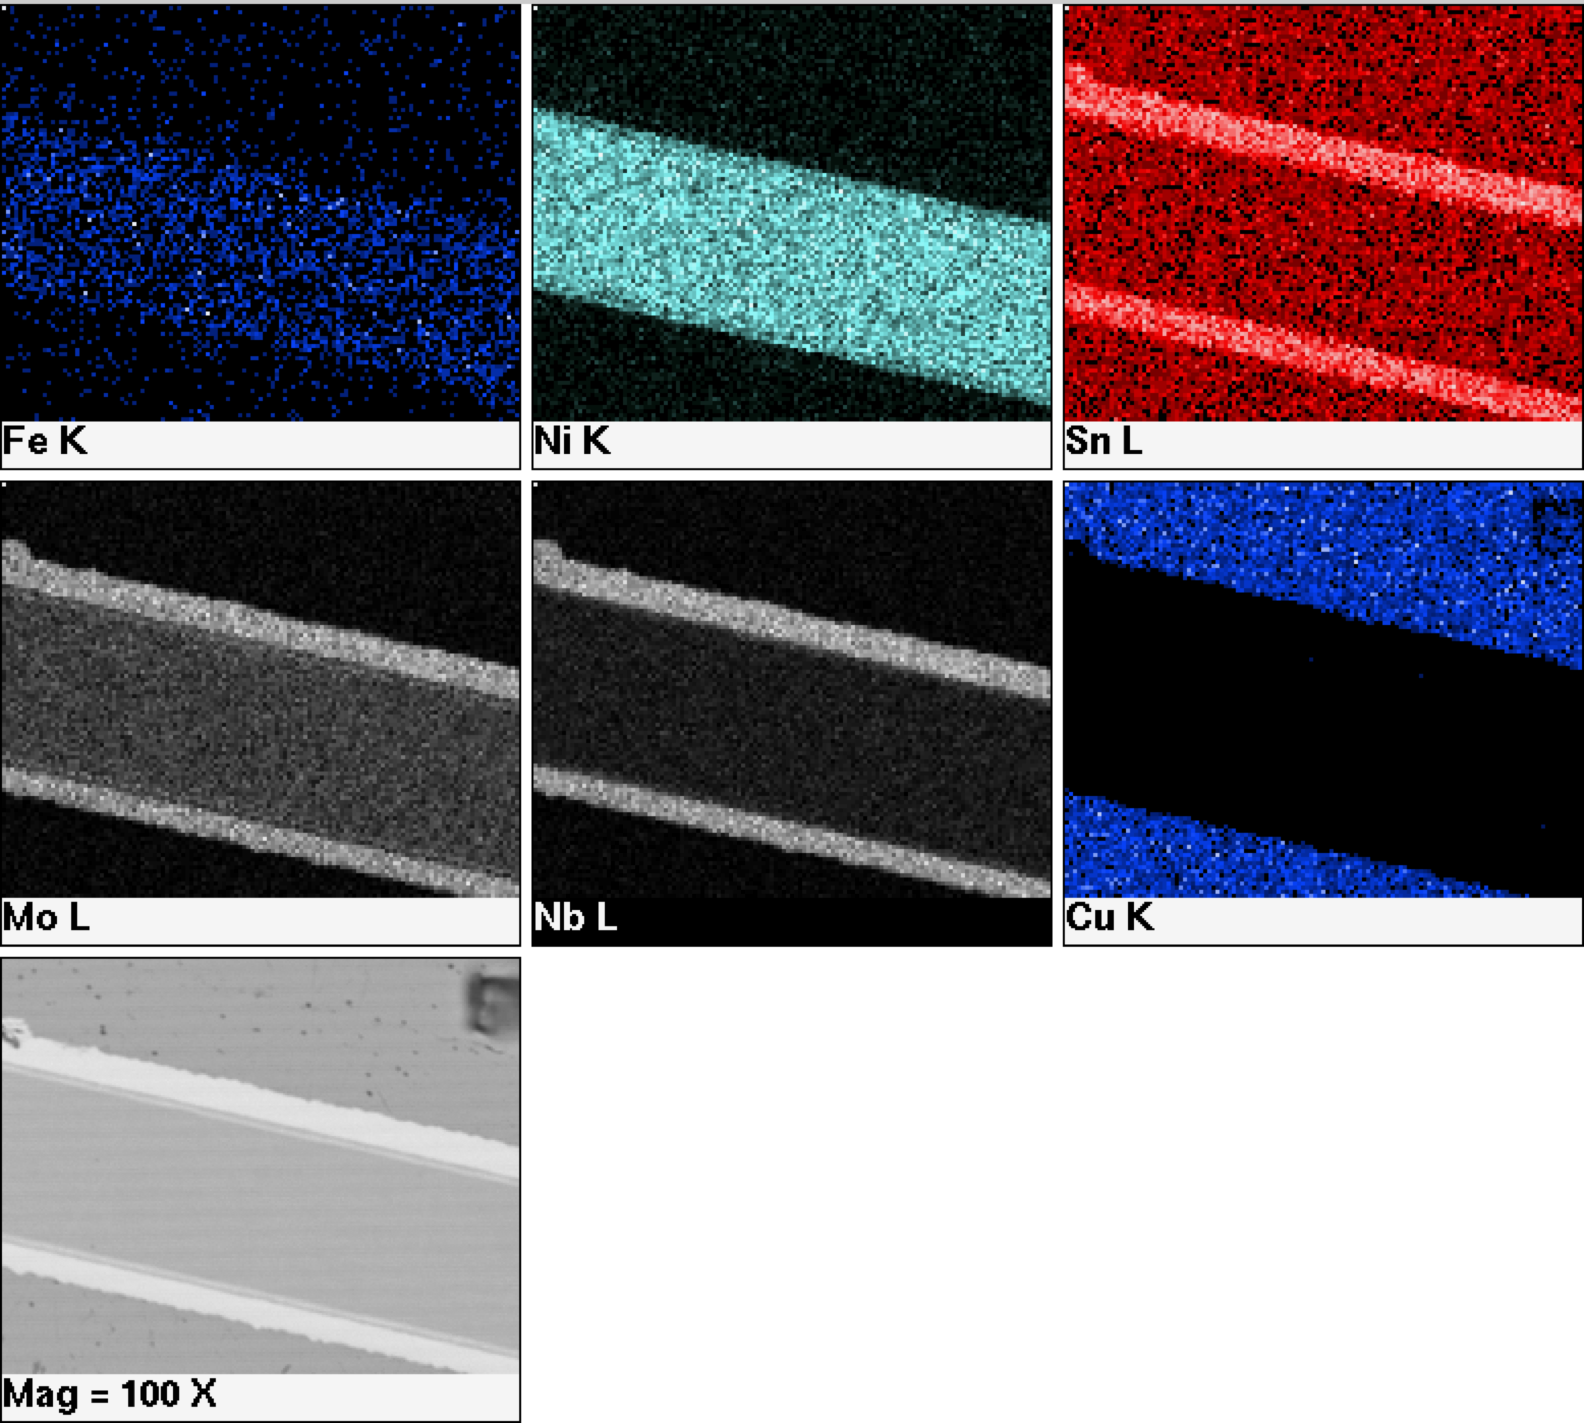
\includegraphics[width=\textwidth]{images/im5.png}
\caption{Images réalisées à l'aide de mesure EDS répétées en différents points de l'échantillon. Un élément est associé à une couleur, la représentation est plus visuelle.}
\label{fig:eds}
\end{figure}





\section*{Conclusion}


On a pu voir lors de ce TP la large gamme de possibilités offerte par la microscopie MEB. En effet, en tirant partie des différents phénomènes physiques, on peut avoir des informations sur la composition chimique, la répartition des composés dans l'espace, l'état de surface, les plans cristallographiques, le relief de l'échantillon. Ses avantages par rapport à la microscopie optique sont aussi non négligeable, la résolution et la profondeur de champs sont par exemple bien meilleure. Et bien que les échantillons observés doivent être conducteur, on arrive, par des techniques de déposition, à permettre l'observation d'échantillons organiques.




\end{document}
